\documentclass[conference]{IEEEtran}
\IEEEoverridecommandlockouts
% The preceding line is only needed to identify funding in the first footnote. If that is unneeded, please comment it out.
% \usepackage{cite}
\usepackage{amsmath,amssymb,amsfonts}
\usepackage{algorithmic}
\usepackage{graphicx}
\graphicspath{ {./images/} }
\usepackage{textcomp}
\usepackage{tikz}
\usepackage{pgfplots}
\usepackage{xcolor}
\usepackage{caption}  

% biblatex
% \usepackage{biblatex}
% \addbibresource{bibtex/PaperDubai.bib}
% \addbibresource{zotero.bib}

\def\BibTeX{{\rm B\kern-.05em{\sc i\kern-.025em b}\kern-.08em
    T\kern-.1667em\lower.7ex\hbox{E}\kern-.125emX}}
\begin{document}

\makeatletter
\newcommand{\linebreakand}{%
    \end{@IEEEauthorhalign}
    \hfill\mbox{}\par
    \mbox{}\hfill\begin{@IEEEauthorhalign}
}
\makeatother

\title{Performance comparison of natural language understanding engines in the educational domain}

\author{\IEEEauthorblockN{1\textsuperscript{st} Víctor Juan Jimenez Flores}
    \IEEEauthorblockA{\
        \textit{Faculty of Engineering} \\
        \textit{Universidad José Carlos Mariátegui}\\
        Moquegua, Perú \\
        victorjuanjf@jfbots.com}
    % asociación peruana de investigación, ciencia y tecnología comprar dominio antes de enviar paper
    \and
    \IEEEauthorblockN{2\textsuperscript{nd} Oscar Juan Jimenez Flores}
    \IEEEauthorblockA{
        \textit{Faculty of Engineering} \\
        \textit{Universidad Privada de Tacna}\\
        Tacna, Perú \\
        oscarjimenezflores@upt.pe}
    \and
    \IEEEauthorblockN{3\textsuperscript{rd} Juan Carlos Jimenez Flores}
    \IEEEauthorblockA{
        \textit{Contracts and services} \\
        \textit{Southern Peru Copper Corporation}\\
        Tacna, Perú \\
        jjimenez@southernperu.com.pe}
    \linebreakand % <------------- \and with a line-break
    \IEEEauthorblockN{4\textsuperscript{th} Juan Ubaldo Jimenez Castilla}
    \IEEEauthorblockA{
        \textit{Faculty of Engineering} \\
        \textit{Universidad José Carlos Mariátegui }\\
        Moquegua, Perú \\
        jjimenez@ujcm.edu.pe}
}

\maketitle

\begin{abstract}
    This research aims to compare the main natural language understanding (NLU) engines and find which one has the highest performance in the educational domain. In this way, researchers can make more justified decisions about which NLU engine to use to develop an educational chatbot. Besides, in this study, six NLU platforms were compared and performance was measured with the F1 score. Training data and input messages were extracted from Mariateguino Bot, which was the chatbot of the José Carlos Mariátegui University during 2018. The results of this comparison indicates that Watson Assistant has the best performance, with an average F1 score of 0.82.

\end{abstract}

\begin{IEEEkeywords}
    chatbot, Natural Language Understanding, NLU, F1 score, performance
\end{IEEEkeywords}

\section{Introduction}
Nowadays, the business and researchers are progressively perceive the importance of chatbot systems, because they are integrated into daily life, playing roles as assistants to end users \cite{Bird2018}. In the educational domain, Kowalski indicates that chatbots can play an important role, because it represents an interactive mechanism, instead of the traditional e-learning systems, where students can constantly ask questions related to a specific field \cite{Kowalski2011}.

On the other hand, most research does not emphasize the used natural language understanding (NLU) engine, or its choice is not very justified. Therefore, this research compares different NLU engines, like Dialogflow, LUIS, Watson Assistant, Wit.ai, Amazon LEX and Rasa (an open source chatbot framework) and tries to answer, in terms of performance and educational domain, which one to use.

A chatbot is a computer program which uses machine learning technique voice recognition, and natural language processing (NLP) to conduct a intelligent conversation with a person (e.g. Amazon's Alexa and Google's Assistant) \cite{mittal2019getting}. Moreover, one of the main components of a chatbot is the natural language understanding (NLU), which is the ability of a machine to understand human languages, said otherwise, it is the process of converting natural language text into a form that computers can understand \cite{pathak2017artificial}.

Besides, in this research, training data and input messages were extracted from Mariateguino Bot,which was the chatbot of the José Carlos Mariátegui University during 2018, its main function was to attend to the doubts of the students regarding the necessary requirements to carry out administrative procedures. Moreover, the chatbot was able to answer frequently asked questions, support students regarding the admissions process, and provide class schedules.

Mariateguino Bot was made with Dialogflow \cite{dialogflow2020}, a Google service that runs on Google Cloud Platform. Therefore, other platforms, described in section \ref{sec:nluServices}, were evaluated.

To determine the performance of the evaluated services, the F1 score was used. F1 score is defined as the harmonic mean of precision and recall \cite{campesato2020artificial} and it was chosen because it is one of the most practical ways to numerically calculate the performance of an NLU engine and it is widely used in related researches. In addition, according to \cite{arnicans2016databases}, using the f1 score, the results can be easily compared with previous works, because it is one of the standard metrics for performance measurement.
% In order to identify F1 score, it was necessary to calculate the precision and recall.

Finally, this paper is divided into seven sections. Section II gives a brief overview of related works. Section III defines the NLU engines evaluated during the research. Section IV describes the methodology. Section V and section IV describe the results and discussions. Finally, section VII and section VIII describe the conclusions and future work.

\section{Related works}
In recent years, many researches have been carried out regarding chatbots and the impact they have on traditional processes, generally in customer service. Some performance related researches are listed below.

Canonico and De Russis wrote a paper titled "A comparison and Critique of Natural Language Understanding Tools" \cite{Canonico2018}, which compares the main cloud-based platforms, from a descriptive and performance based point of view. Their results showed that Watsson Assistant is the platform who performs best.

On the other hand, Braun, Hernandez, Matthes and Langen wrote a paper titles "Evaluating Natural Language Understanding Services for Conversational Question Answering Systems", which presents a method to evaluate the classification performance of NLU services. Their results indicated that LUIS showed the best scores and RASA could achieve similar results.

\section{Natural language understanding engines} \label{sec:nluServices}
There are many natural language understanding modules that are available as cloud services and major IT players like Google, Microsoft, IBM, Facebook and Amazon have created tools to develop chatbots \cite{hall2017hands}. Additionally, Rasa was included because Dialogflow training data can be converted to its format and is an open source alternative compared to the other platforms.
\subsection{Dialogflow}
Dialogflow is a Google's bot engine that runs on Google Cloud Platform. Similarly, Dialogflow is a natural language understanding platform that makes it easy to design and integrate a conversational user interface into any system \cite{dialogflow2020}.
\subsection{LUIS}
The Language Understanding Intelligent Service (LUIS) is a Microsoft's bot engine that runs on Azure Cognitive Services \cite{pathak2018iot}.
\subsection{Watsson Assistant}
Watsson Assistant a IBM's bot engine which makes it easy to create conversational interfaces and integrates them into any application \cite{sabharwal2019developing}.
\subsection{Wit.ai}
Wit.ai is a Facebook's bot engine which allows training bots with sample conversations and have your bots repeatedly learn from interrelating with customers \cite{seligman2018artificial}.
\subsection{Amazon LEX}
Amazon Lex is a Amazon's bot engine for building intelligent assistants or chatbots, which provides many AI capabilities like Automatic Speech Recognition (ASR) and Natural language Understanding (NLU) \cite{tripuraneni2019hands}.
\subsection{Rasa}
Rasa NLU is an open-source NLP library for intent classification and entity extraction in chatbots \cite{raj2018building}.

\section{Methods}
The method of evaluating the classification performance of NLU engines is based on \cite{Braun2017}.
\subsection{Materials}
The NLU engines evaluated during the research were Dialogflow, Wit.ai, LUIS, Amazon LEX and Rasa. Moreover, 100 messages from the Mariateguino Bot conversation history were selected as input data and they were grouped based on the expected intents, thus obtaining 30 intents. To calculate the performance of each platform, the F1 score metric was used, which includes precision and recall.

\subsection{Procedure}
The experimental design, indicated below, is based on \cite{Braun2017}.

As a first step, a conversion of the Dialogflow training data to the rest of the research platforms was carried out, using the QBox.ai service \cite{qbox2020}. Then, one hundred messages were randomly selected from Mariateguino Bot conversation history and they were grouped based on the expected intents, thus obtaining 30 intents.

Afterwards, to start testing and obtain data, a Node.js application was created in order to combine the application programming interface (API) from each NLU engine, in such a way that each input message was only entered once and the desired data was obtained in the format shown in Fig. \ref{fig:nludata}. Also, a threshold of 0.5 was programmed for all platforms, so that if the API of the NLU engine returns a confidence less than 0.5, the Node.js application returns the default fallback intent.

\begin{figure}[t]
    \centerline{\fbox{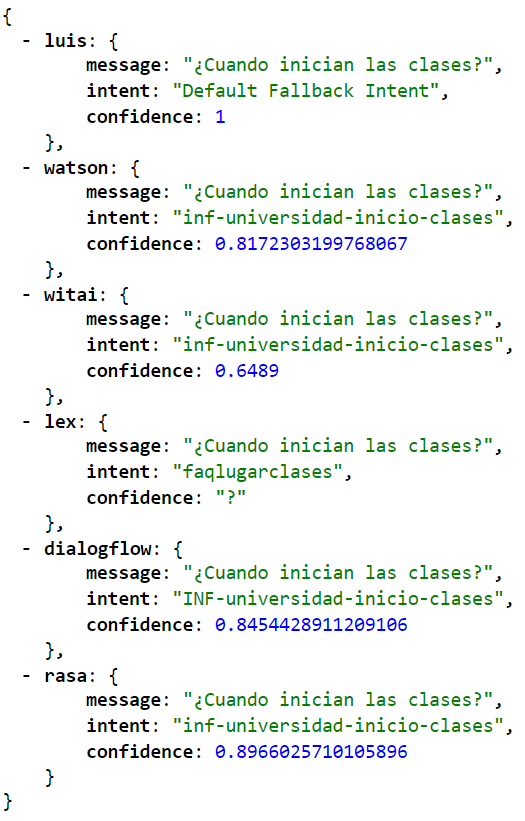
\includegraphics[scale=0.58,height=11.3cm]{nlu}}}
    \caption{Node.js application output}
    \label{fig:nludata}
\end{figure}

In order to evaluate the results, the predicted intent were identified for each input message. In this way, true positives (TP), false positives (FP) and false negatives (FN) were calculated.

As a final step, the performance of the NLU engines was measure in terms of precision, recall and F1 score, given by the following expressions:

\begin{equation}
    Precision=\frac{TP}{TP+FP}\label{eq1}
\end{equation}
\begin{equation}
    Recall=\frac{TP}{TP+FN}\label{eq2}
\end{equation}
F1 score is defined as the harmonic mean of precision and recall \cite{campesato2020artificial}.
\begin{equation}
    F_{1} =\frac{2 \times Precision\times Recall}{Precision+Recall}\label{eq3}
\end{equation}

These measures were applied for single intents, then the average F1 score was calculated. For this research, one NLU engine is better than another if it has a higher average F1 score.

\section{Results}

The results shown in Fig. \ref{fig:precision}, Fig. \ref{fig:recall}, Fig. \ref{fig:f1score} and table \ref{tab:overview} are the average precision, recall and F1 score of the 30 intents that were evaluated for each natural language understanding engine.

In terms of precision, as Fig. \ref{fig:precision} shows, Dialogflow has the highest value (0.83), while LUIS obtained the lowest value (0.46).

In terms of recall, as Fig. \ref{fig:precision} shows, Watson Assistant has the highest value (0.89), while LUIS obtained the lowest value (0.34).

Finally, in terms of F1 score, calculated from precision and recall, as Fig. \ref{fig:precision} shows, Watson Assistant and Dialogflow have the highest value (0.82), while LUIS obtained the lowest value (0.36).

Overall, as can be seen in Table \ref{tab:overview}, Watson Assistant and Dialogflow performed better, while LUIS obtained the lowest performance.

\begin{figure}[hp]
    \begin{center}
        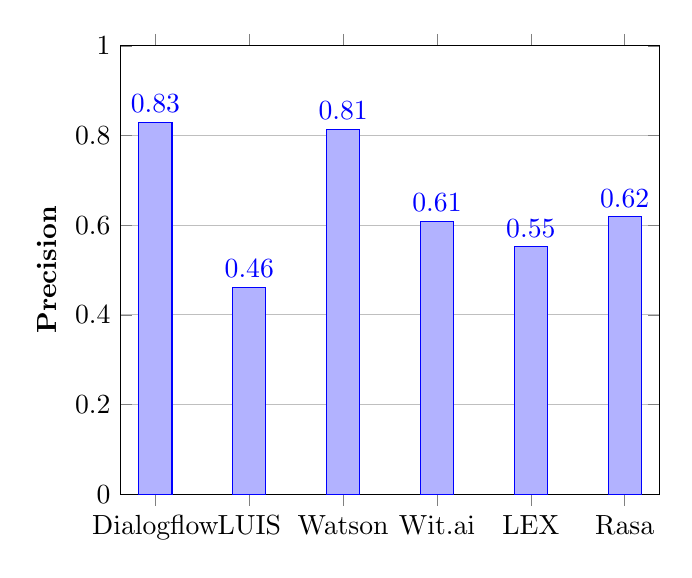
\begin{tikzpicture}
            \begin{axis}
                [
                    ybar,
                    bar width=12pt,
                    ylabel=Precision,
                    % xlabel=NLU services,
                    symbolic x coords={Dialogflow,LUIS,Watson,Wit.ai,LEX,Rasa},
                    enlarge x limits=0.075,
                    xtick=data,
                    xmajorgrids = false,
                    ymajorgrids = true,
                    ymin=0,
                    ymax=1,
                    % axis y line = left,
                    every outer y axis line/.append style = {-},
                    every outer x axis line/.append style = {-},
                    ylabel style = {font=\bfseries},
                    xlabel style = {font=\bfseries},
                    nodes near coords,
                    nodes near coords align={vertical},
                ]
                \addplot coordinates {(Dialogflow,0.828333333) (LUIS,0.461717171717172) (Watson,0.813918128654971) (Wit.ai,0.607663117663118) (LEX,0.551633986928105) (Rasa,0.618515325670498) };
            \end{axis}
        \end{tikzpicture}
        \captionof{figure}{Precision of natural language understanding engines}
        \label{fig:precision}
    \end{center}
\end{figure}
\begin{figure}[hp]
    \begin{center}
        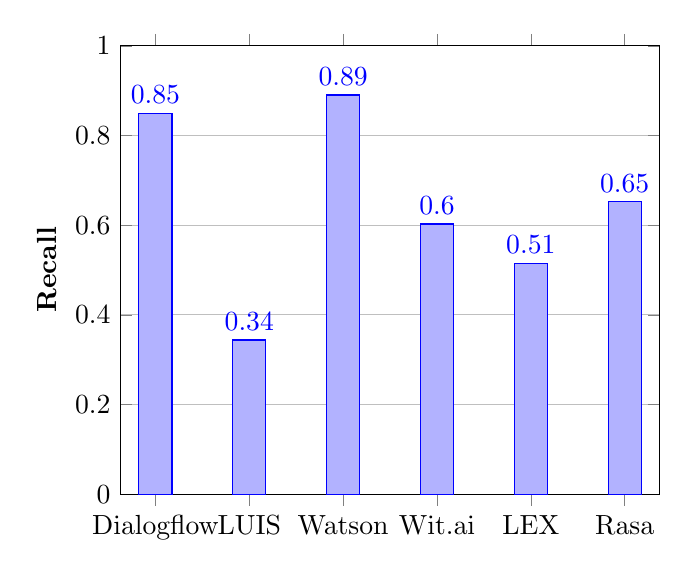
\begin{tikzpicture}
            \begin{axis}
                [
                    ybar,
                    bar width=12pt,
                    ylabel=Recall,
                    % xlabel=NLU services,
                    symbolic x coords={Dialogflow,LUIS,Watson,Wit.ai,LEX,Rasa},
                    enlarge x limits=0.075,
                    xtick=data,
                    xmajorgrids = false,
                    ymajorgrids = true,
                    ymin=0,
                    ymax=1,
                    % axis y line = left,
                    every outer y axis line/.append style = {-},
                    every outer x axis line/.append style = {-},
                    ylabel style = {font=\bfseries},
                    xlabel style = {font=\bfseries},
                    nodes near coords,
                    nodes near coords align={vertical},
                ]
                \addplot coordinates {(Dialogflow,0.848744588744589) (LUIS,0.343726551226551) (Watson,0.89017316017316) (Wit.ai,0.602640692640693) (LEX,0.514170274170274) (Rasa,0.651991341991342) };
            \end{axis}
        \end{tikzpicture}
        \captionof{figure}{Recall of natural language understanding engines}
        \label{fig:recall}
    \end{center}
\end{figure}
\begin{figure}[hp]
    \begin{center}
        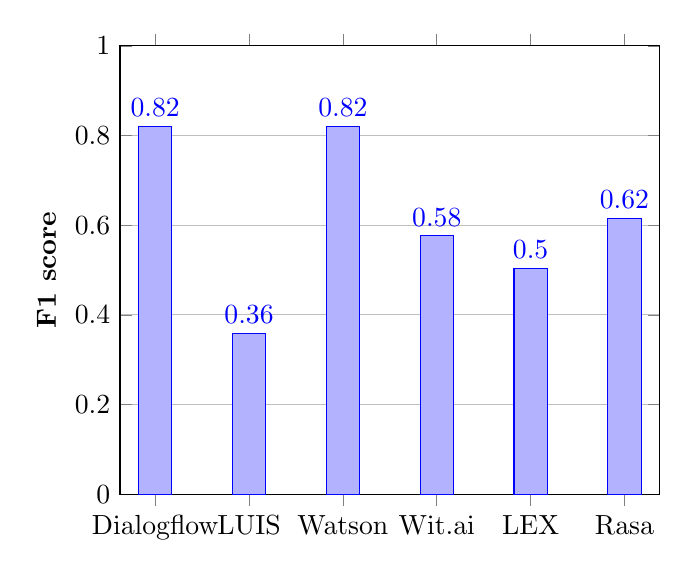
\begin{tikzpicture}
            \begin{axis}
                [
                    ybar,
                    bar width=12pt,
                    ylabel=F1 score,
                    % xlabel=NLU services,
                    symbolic x coords={Dialogflow,LUIS,Watson,Wit.ai,LEX,Rasa},
                    enlarge x limits=0.075,
                    xtick=data,
                    xmajorgrids = false,
                    ymajorgrids = true,
                    ymin=0,
                    ymax=1,
                    % axis y line = left,
                    every outer y axis line/.append style = {-},
                    every outer x axis line/.append style = {-},
                    ylabel style = {font=\bfseries},
                    xlabel style = {font=\bfseries},
                    nodes near coords,
                    nodes near coords align={vertical},
                ]
                \addplot coordinates {(Dialogflow,0.820630111) (LUIS,0.357854738
                        ) (Watson,0.820979481) (Wit.ai,0.576004394) (LEX,0.503356458) (Rasa,0.615315904) };
            \end{axis}
        \end{tikzpicture}
    \end{center}
    \captionof{figure}{F1 score of natural language understanding engines}
    \label{fig:f1score}
\end{figure}

\begin{table}[hp]
    \caption{F1 scores overview}
    \begin{center}
        \begin{tabular}{|c|c|c|c|}
            \hline
            \textbf{NLU Engine} & \textbf{Precision} & \textbf{Recall} & \textbf{F1 score} \\
            \hline
            Dialogflow          & 0.83               & 0.85            & 0.82              \\
            \hline
            LUIS                & 0.46               & 0.34            & 0.35              \\
            \hline
            Watson Assistant    & 0.81               & 0.89            & 0.82              \\
            \hline
            Wit.ai              & 0.61               & 0.60            & 0.58              \\
            \hline
            Amazon LEX          & 0.55               & 0.51            & 0.50              \\
            \hline
            Rasa                & 0.62               & 0.65            & 0.62              \\
            \hline
        \end{tabular}%
        \label{tab:overview}%
    \end{center}
\end{table}%
\section{Discussion}

Despite the fact that Watson Assistant and Dialogflow obtained the same F1 score, Watson Assistant can be considered performed best because the original service with which the chatbot was in production was Dialogflow, so it was constantly improving only on that service.

On the other hand, the lower performance of LUIS may be due to the language. Mariateguino Bot was a chatbot made for students in the Spanish language and, despite the fact that LUIS has Spanish in its configuration, it was observed that the intent classification decreases considerably in the presence of input messages that have words with a Spanish accent.

Lastly, the final goal of this research was to compare the main natural language understanding engines and determine which one has the highest performance in the educational domain. Watson assistant was the service with the highest performance; however, for \cite{Braun2017}, LUIS showed the best results. This difference may be due to the fact that the chatbot domain and language was not the same. Moreover, we agree that Rasa can get better results, after some customization, because, during the present research, its full potential as an open source solution was not exploited. In addition, we agree with \cite{Canonico2018}, which indicates that Watson is the platform that performs best since it can assign the correct intention in most of the cases studied, with a high confidence level.

\section{Conclusion}

This study presented a performance comparison of Dialogflow, LUIS, Watson Assistant, Wit.ai, Amazon LEX and Rasa  services in the educational domain, in order to determine which chatbot solution performs best and provide future researchers with more information on which service to choose. It was concluded that Watson Assistant showed the best performance. On the other hand, the performance obtained by Rasa can be considerably improved with the appropriate settings, keeping in mind that it is an open source chatbot framework with a powerful natural language understanding engine.

However, other factors may affect the choice of a platform that provides the NLU engine, such as the level of usability of the service or pricing plans. Therefore, it will be the company or researcher who decides which service best suits their needs.

\section{Future work}

As future work, we plan to evaluate the performance of NLU engines across multiple domains. Similarly, we plan to evaluate the optimal threshold in order to improve performance, since for this research, we only worked with 0.5.


\section*{Acknowledgment}

We would like to thank the José Carlos Mariátegui University, for allowing us to put Mariateguino Bot into production, and its students for their feedback.

\bibliographystyle{IEEEtran}
% \printbibliography
\bibliography{C:/Users/JIMENEZ/Documents/bibtex/PaperIEEE.bib}

\end{document}